
% The environment used here (theappendices) is a wrapper for the basic appendices environment which changes the appearance of the title page and the structure and appearance of the appendices in the table of contents and PDF bookmarks. The original functionality can be restored by simply removing the 'the' from the \begin{} and \end{} statements below.

\begin{theappendices}

	\chapter{Test environments}\label{annexe:cartes}

		\begin{figure}[H]
			\centering
			\begin{subfigure}[t]{\linewidth}
				\centering
				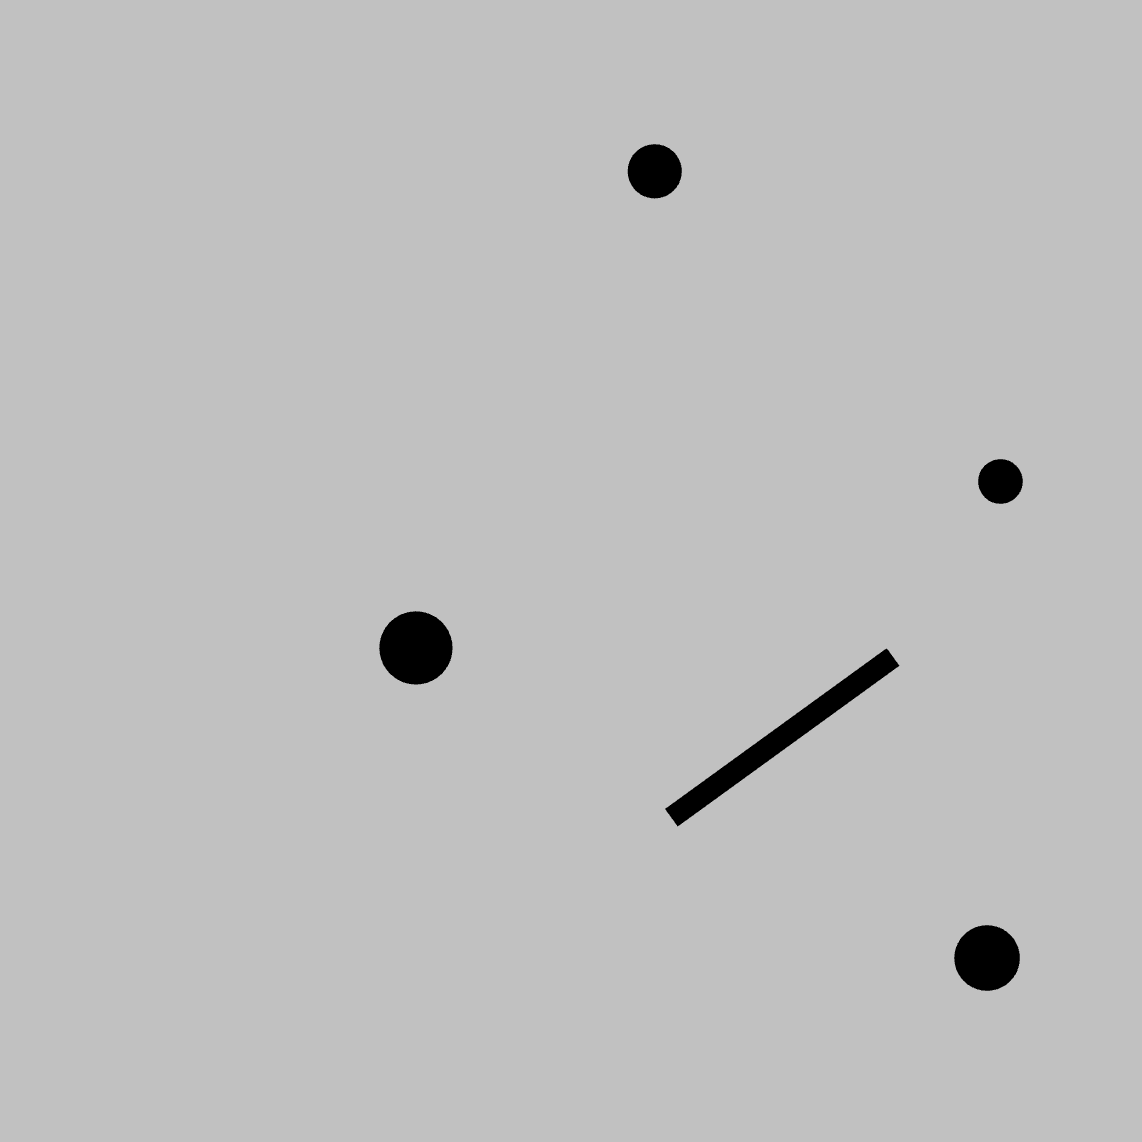
\includegraphics[width=0.15\linewidth]{graphics/test_model_05_1.png}
				\hfill
				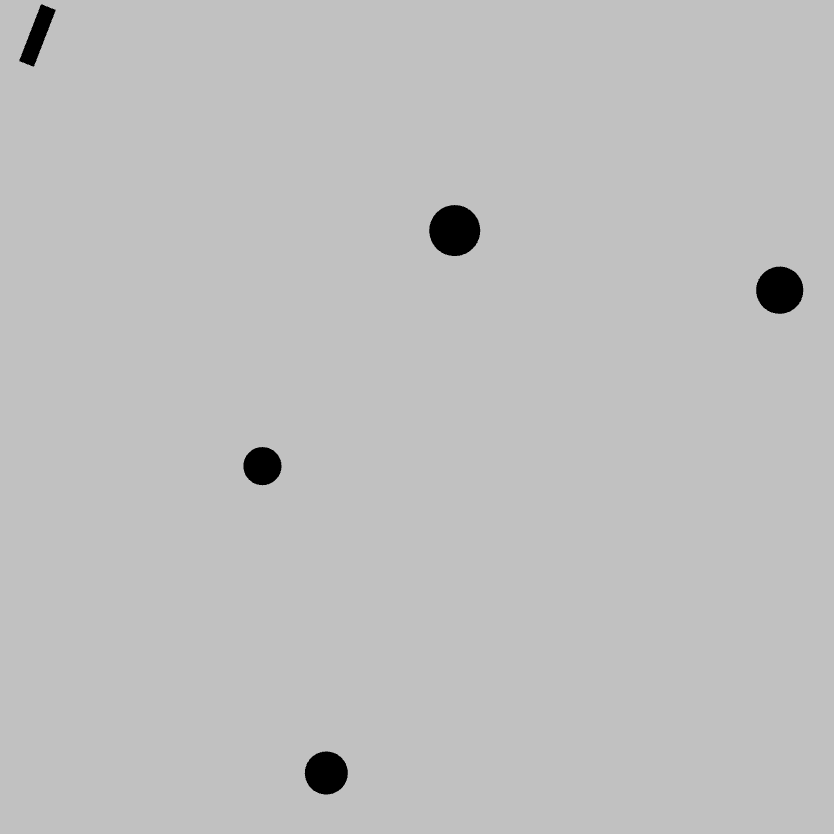
\includegraphics[width=0.15\linewidth]{graphics/test_model_05_2.png}
				\hfill
				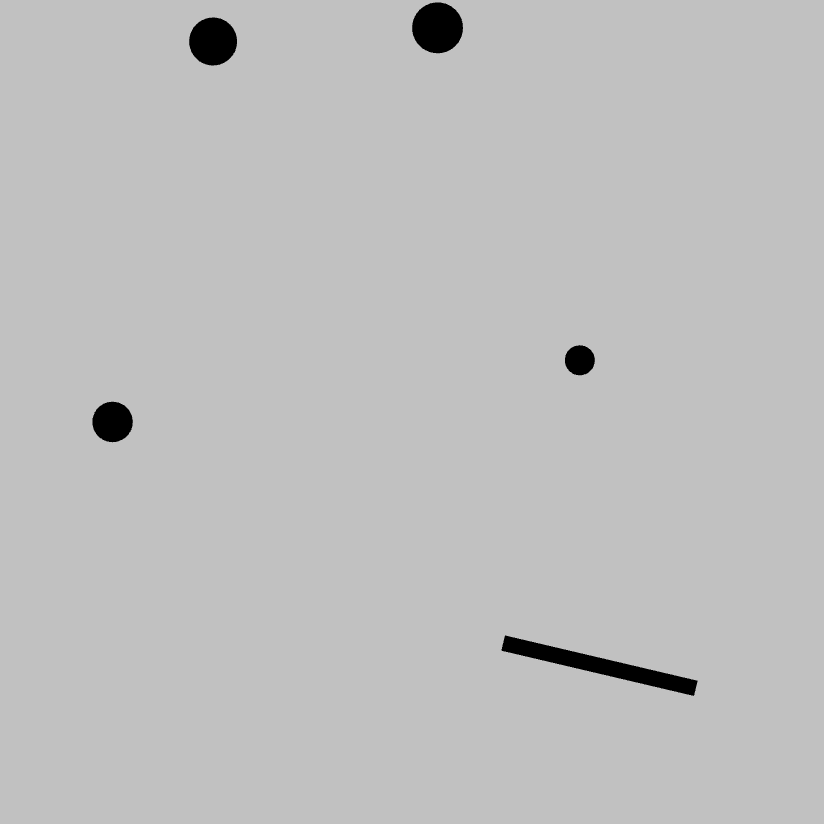
\includegraphics[width=0.15\linewidth]{graphics/test_model_05_3.png}
				\hfill
				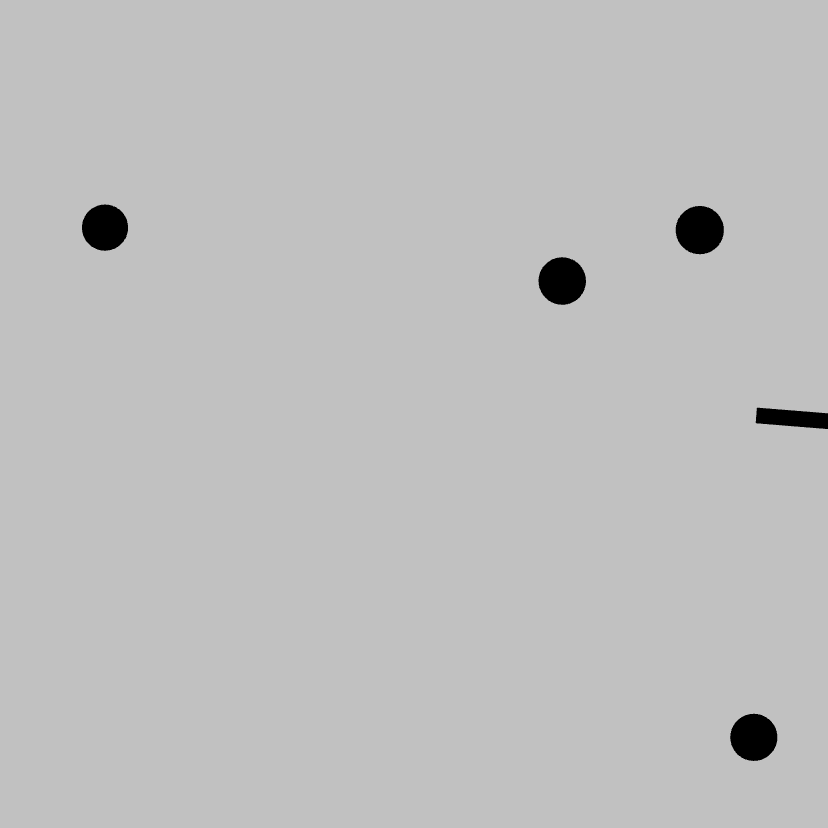
\includegraphics[width=0.15\linewidth]{graphics/test_model_05_4.png}
				\hfill
				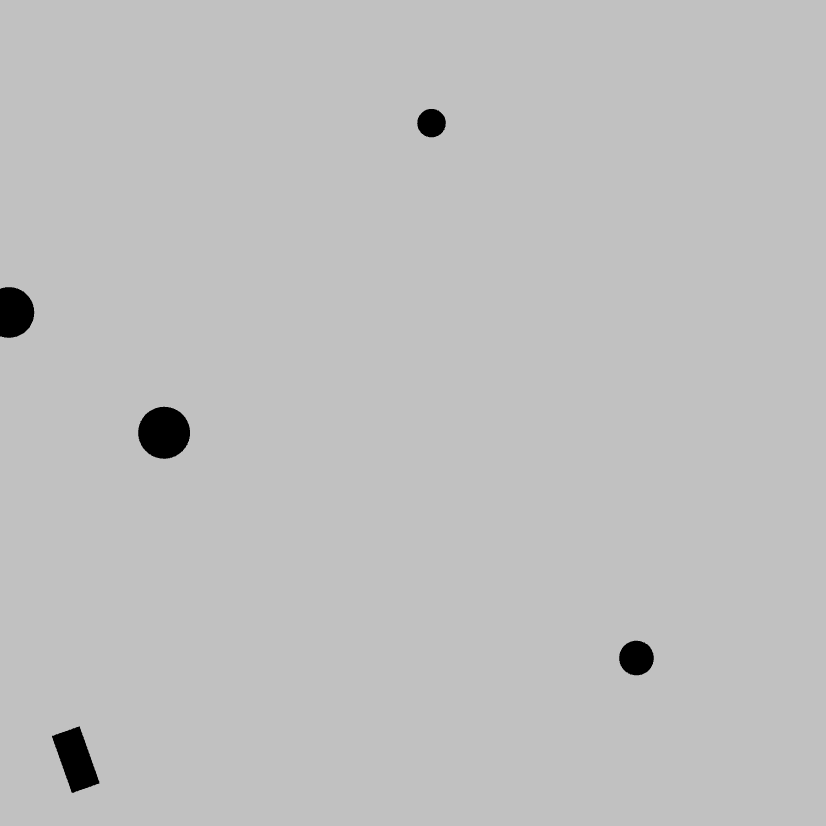
\includegraphics[width=0.15\linewidth]{graphics/test_model_05_5.png}
				\caption{Test worlds with 5 corrosion zones.}
				\label{fig:test_model_05_5}
			\end{subfigure}
			\hfill
			\begin{subfigure}[t]{\linewidth}
				\centering
				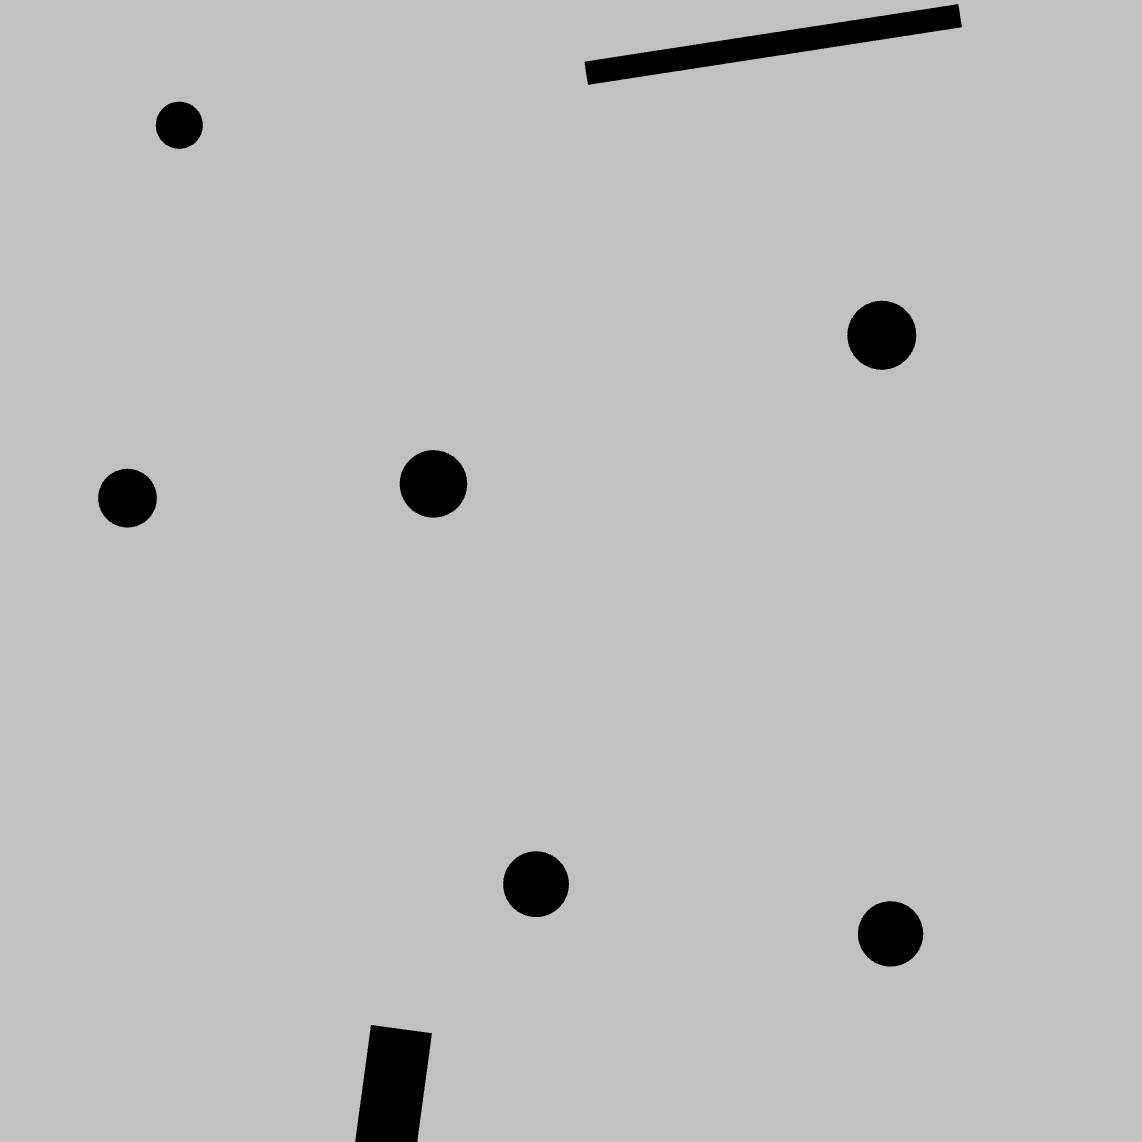
\includegraphics[width=0.15\linewidth]{graphics/test_model_08_1.png}
				\hfill
				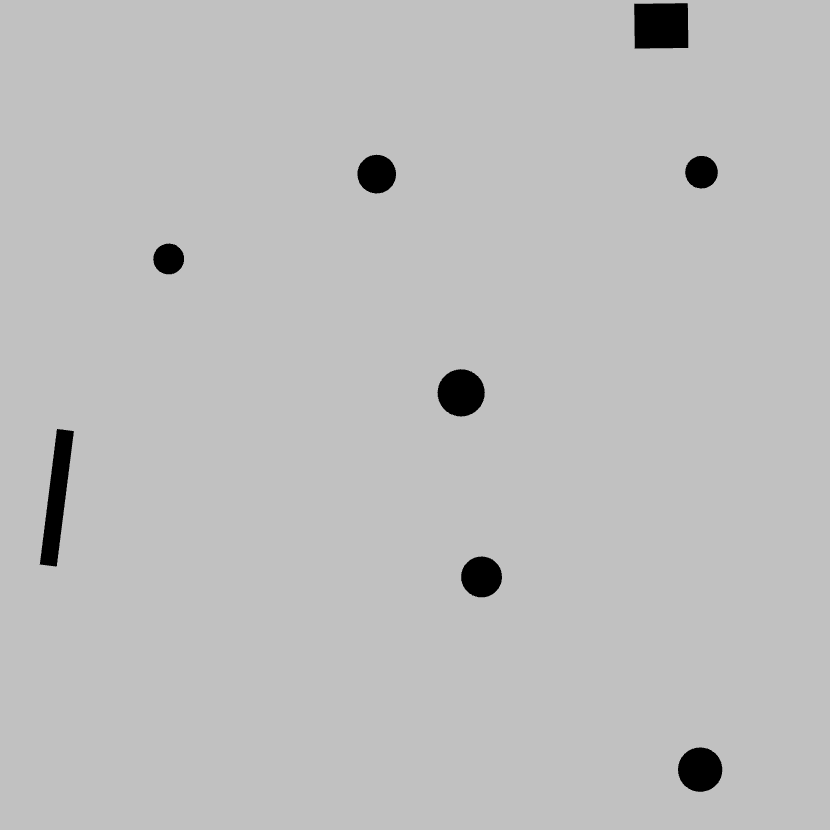
\includegraphics[width=0.15\linewidth]{graphics/test_model_08_2.png}
				\hfill
				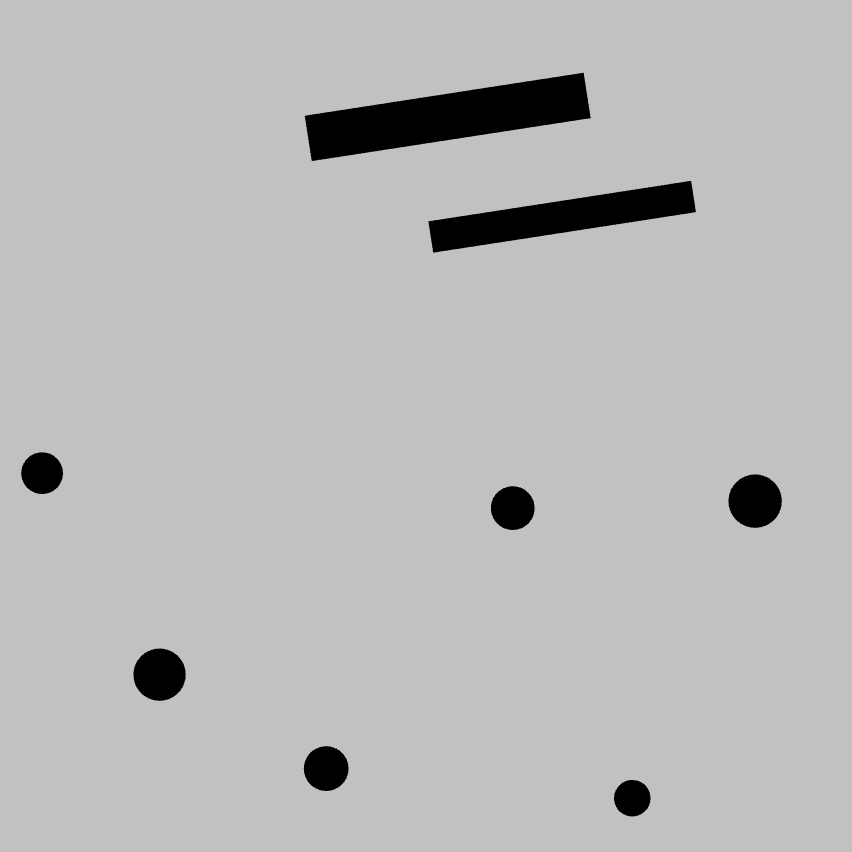
\includegraphics[width=0.15\linewidth]{graphics/test_model_08_3.png}
				\hfill
				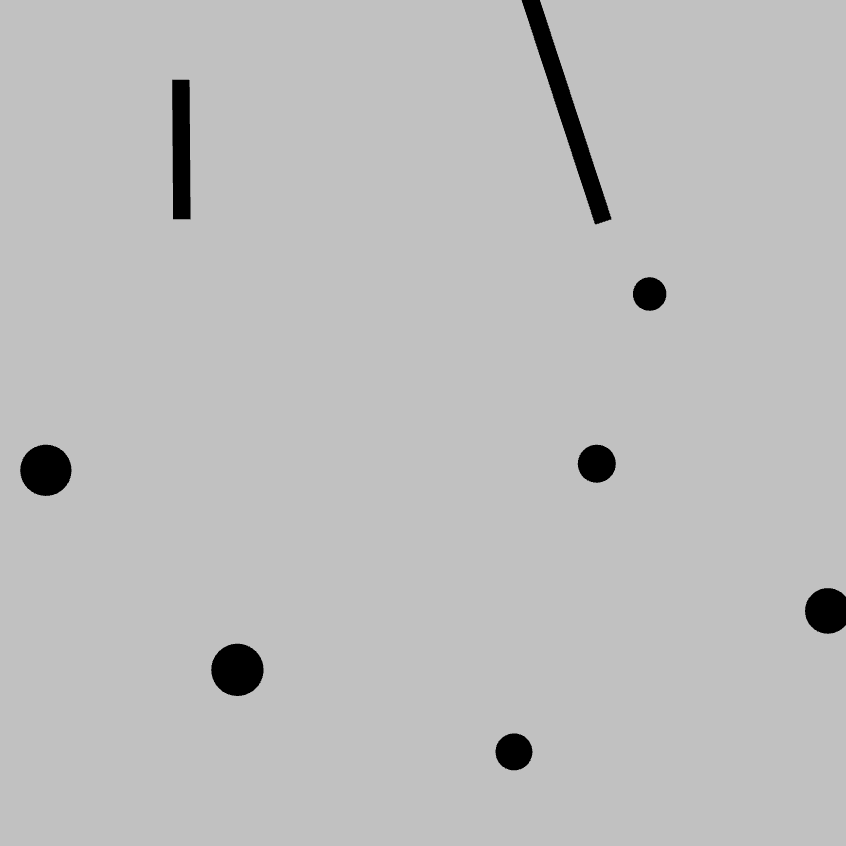
\includegraphics[width=0.15\linewidth]{graphics/test_model_08_4.png}
				\hfill
				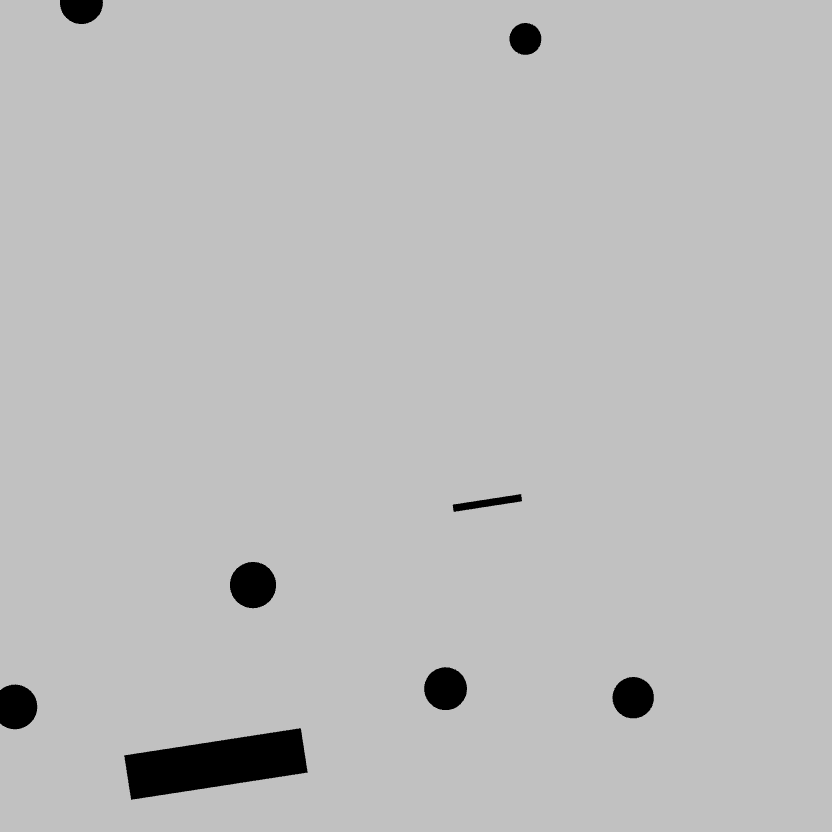
\includegraphics[width=0.15\linewidth]{graphics/test_model_08_5.png}
				\caption{Test worlds with 8 corrosion zones.}
				\label{fig:test_model_08_5}
			\end{subfigure}
			\hfill
			\begin{subfigure}[t]{\linewidth}
				\centering
				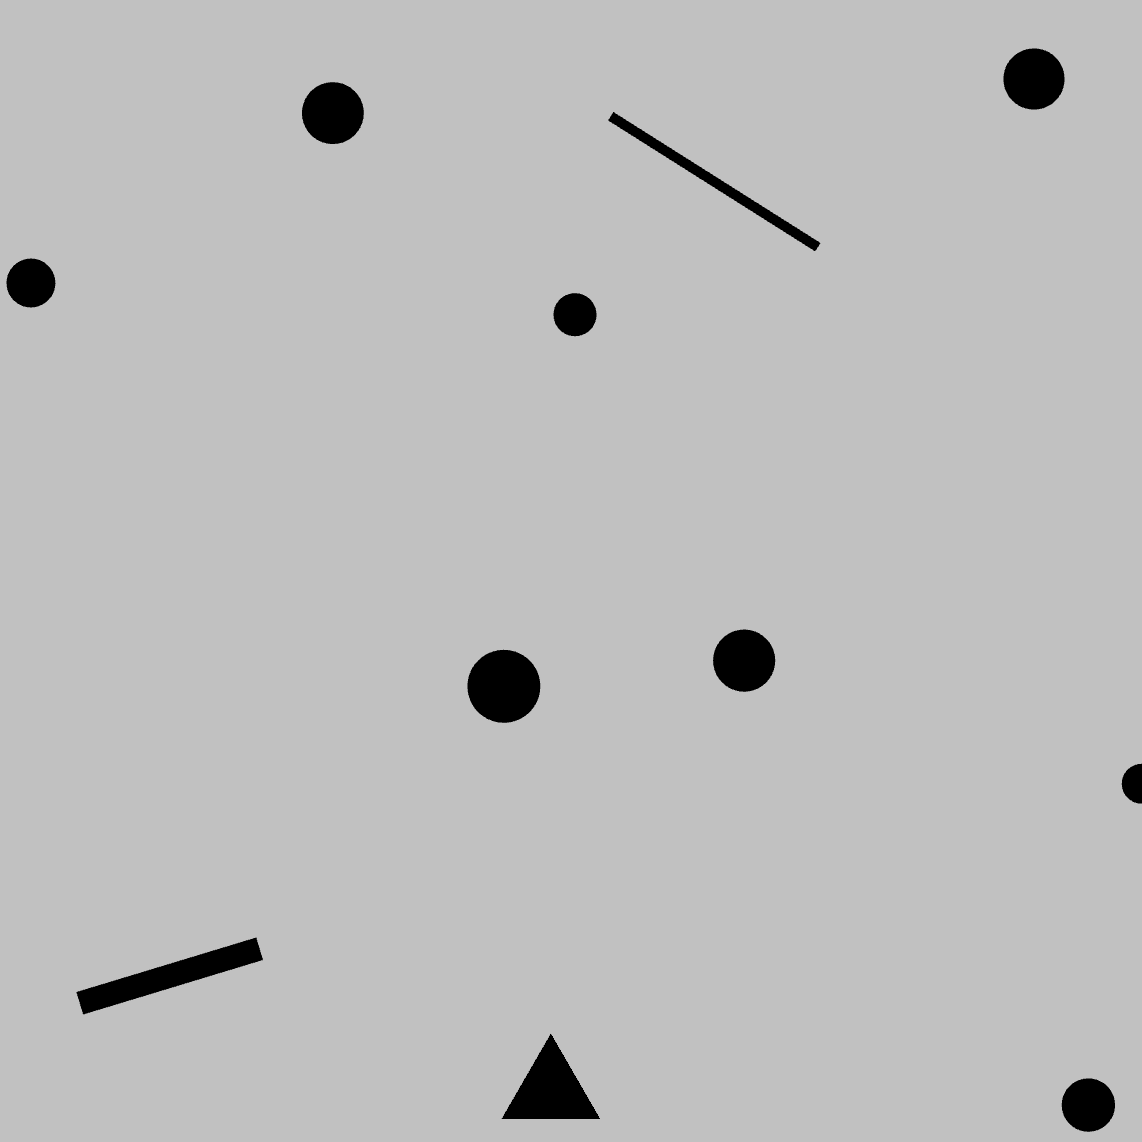
\includegraphics[width=0.15\linewidth]{graphics/test_model_11_1.png}
				\hfill
				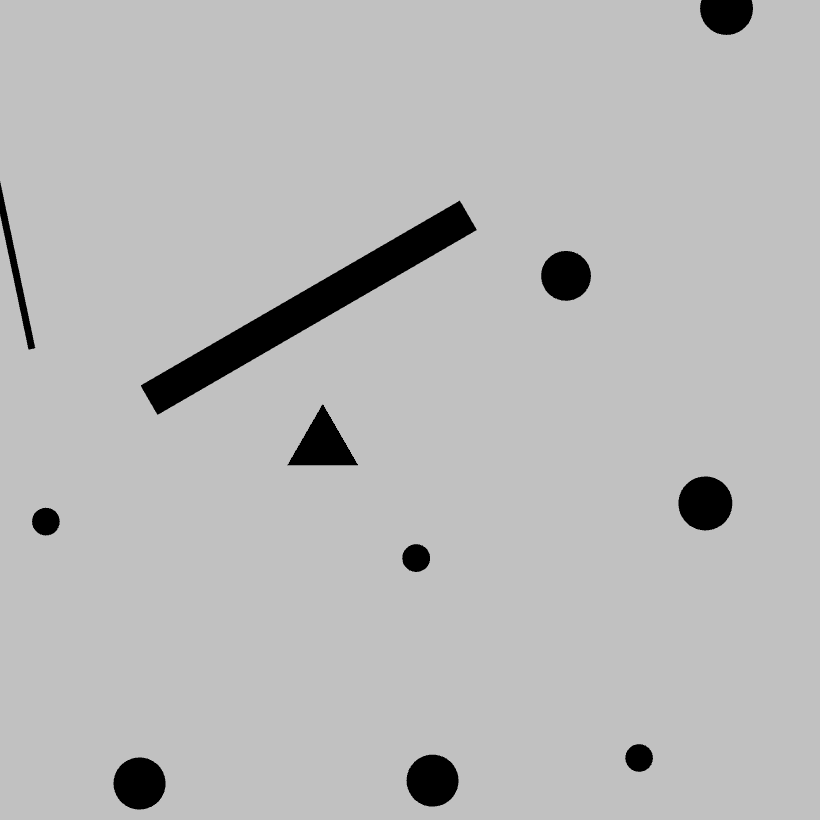
\includegraphics[width=0.15\linewidth]{graphics/test_model_11_2.png}
				\hfill
				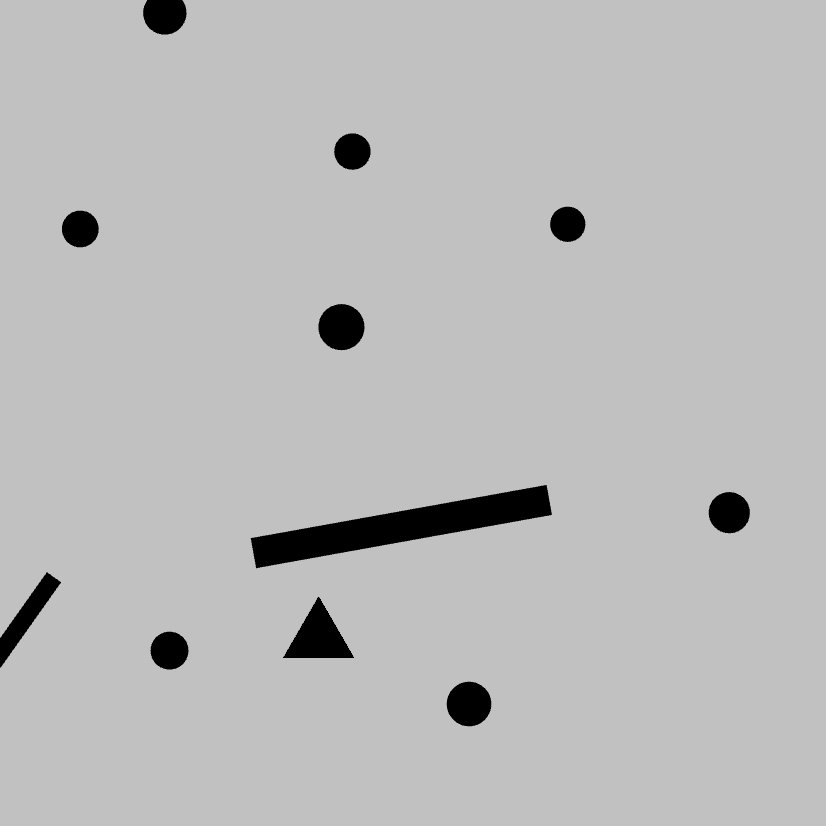
\includegraphics[width=0.15\linewidth]{graphics/test_model_11_3.png}
				\hfill
				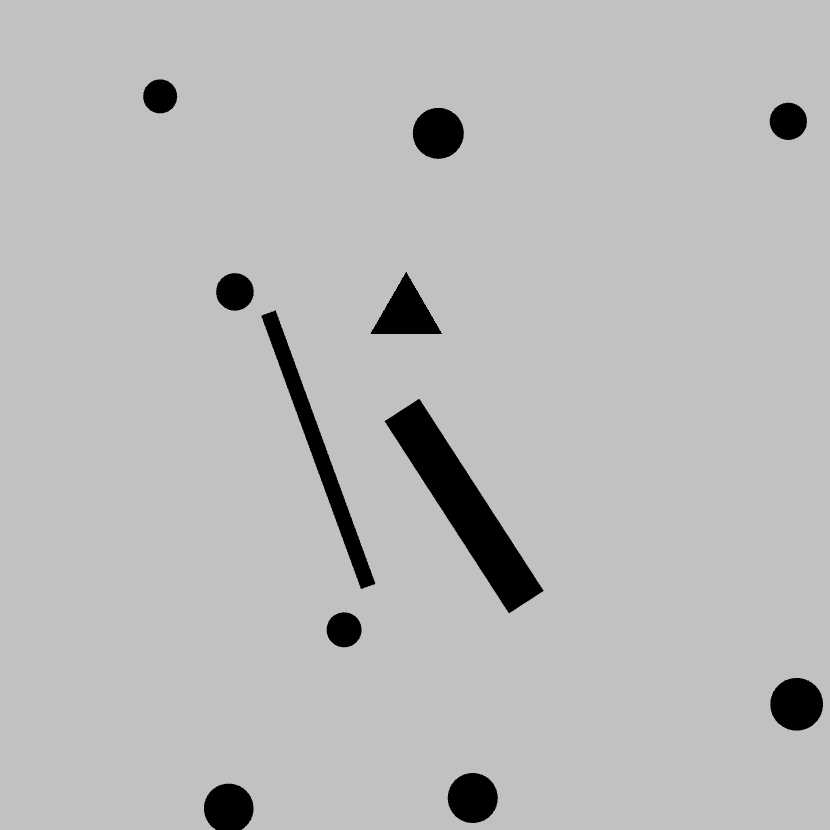
\includegraphics[width=0.15\linewidth]{graphics/test_model_11_4.png}
				\hfill
				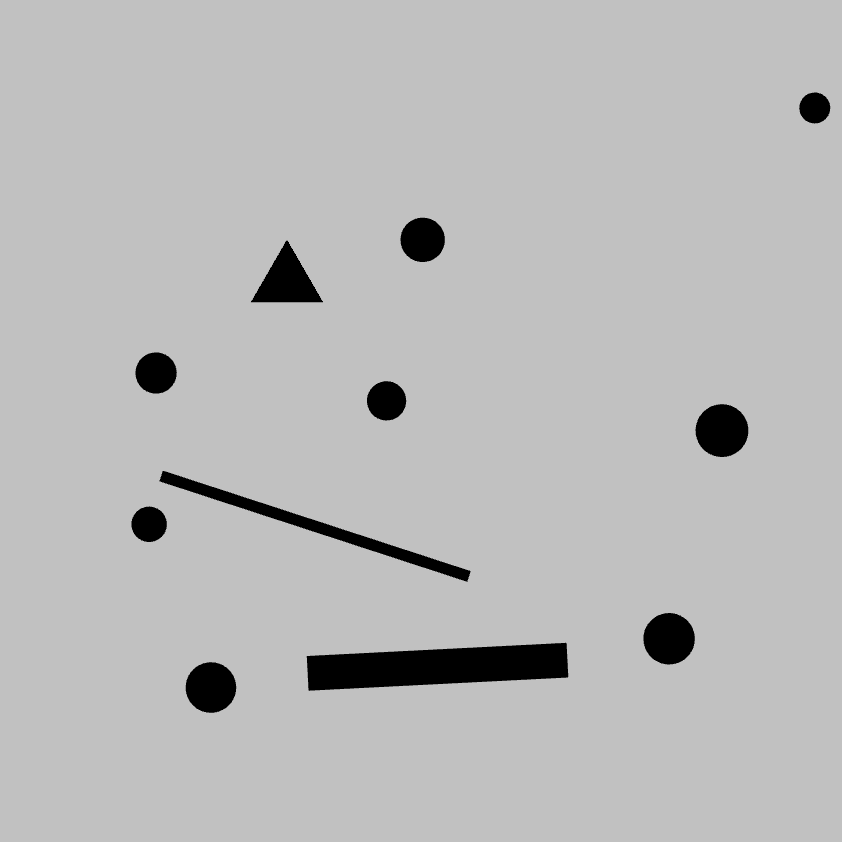
\includegraphics[width=0.15\linewidth]{graphics/test_model_11_5.png}
				\caption{Test worlds with 11 corrosion zones.}
				\label{fig:test_model_11_5}
			\end{subfigure}
			\hfill
			\begin{subfigure}[t]{\linewidth}
				\centering
				
\includegraphics[width=0.15\linewidth]{graphics/test_model_15_1.png}
				\hfill
				
\includegraphics[width=0.15\linewidth]{graphics/test_model_15_2.png}
				\hfill
				
\includegraphics[width=0.15\linewidth]{graphics/test_model_15_3.png}
				\hfill
				
\includegraphics[width=0.15\linewidth]{graphics/test_model_15_4.png}
				\hfill
				
\includegraphics[width=0.15\linewidth]{graphics/test_model_15_5.png}
				\caption{Test worlds with 15 corrosion zones.}
				\label{fig:test_model_15_5}
			\end{subfigure}
			\hfill
			\begin{subfigure}[t]{0.15\linewidth}
				\centering
				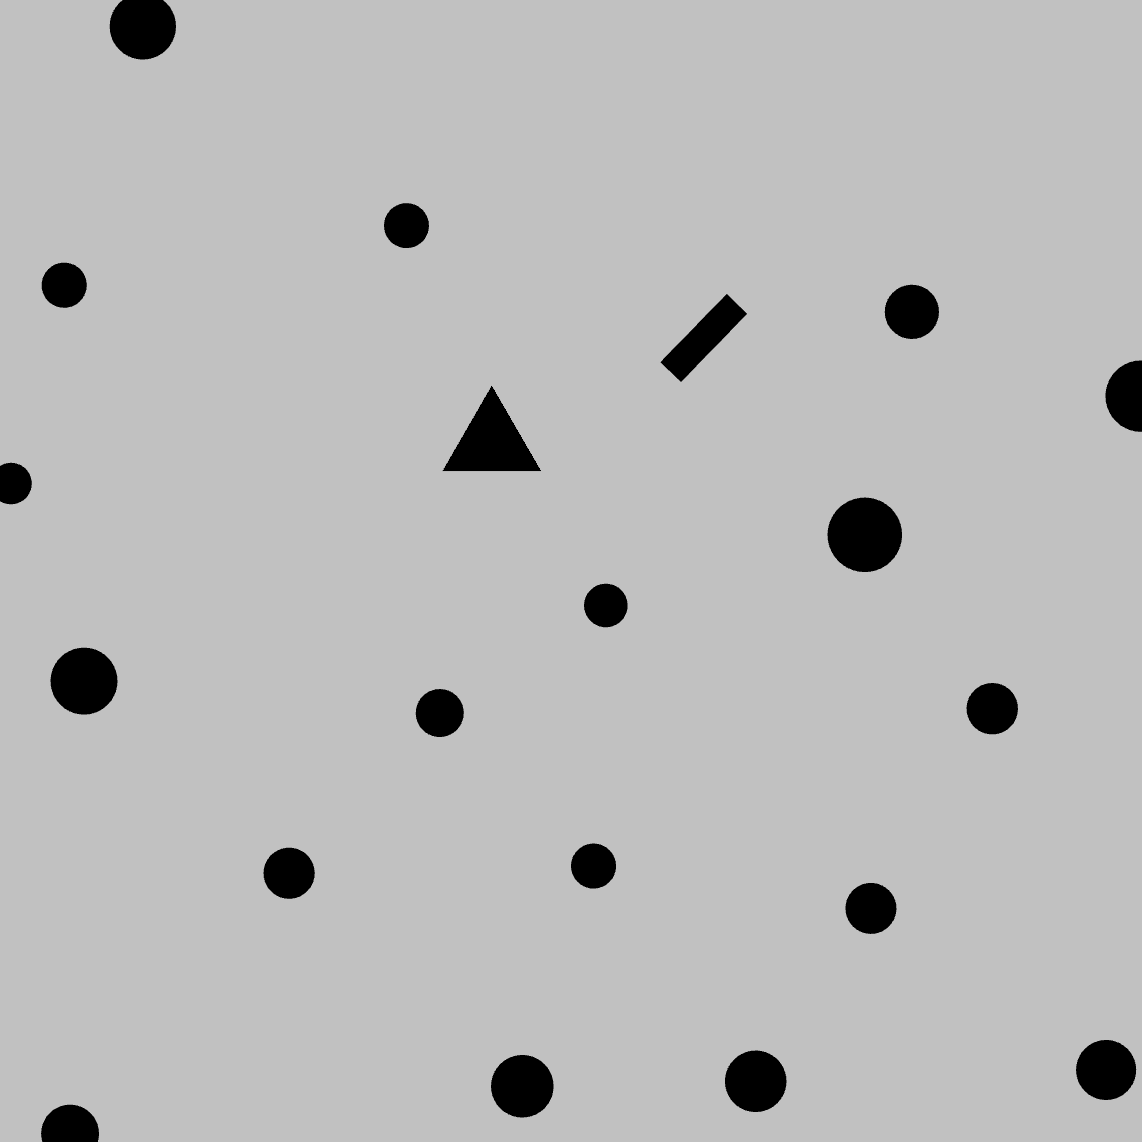
\includegraphics[width=\linewidth]{graphics/test_model_20_1.png}
				\caption{Test worlds with 20 corrosion zones.}
				\label{fig:test_model_20_1}
			\end{subfigure}
			\hfill
			\begin{subfigure}[t]{0.15\linewidth}
				\centering
				
\includegraphics[width=\linewidth]{graphics/test_model_30_1.png}
				\caption{Test worlds with 30 corrosion zones.}
				\label{fig:test_model_30_1}
			\end{subfigure}
			\hfill
			\begin{subfigure}[t]{0.15\linewidth}
				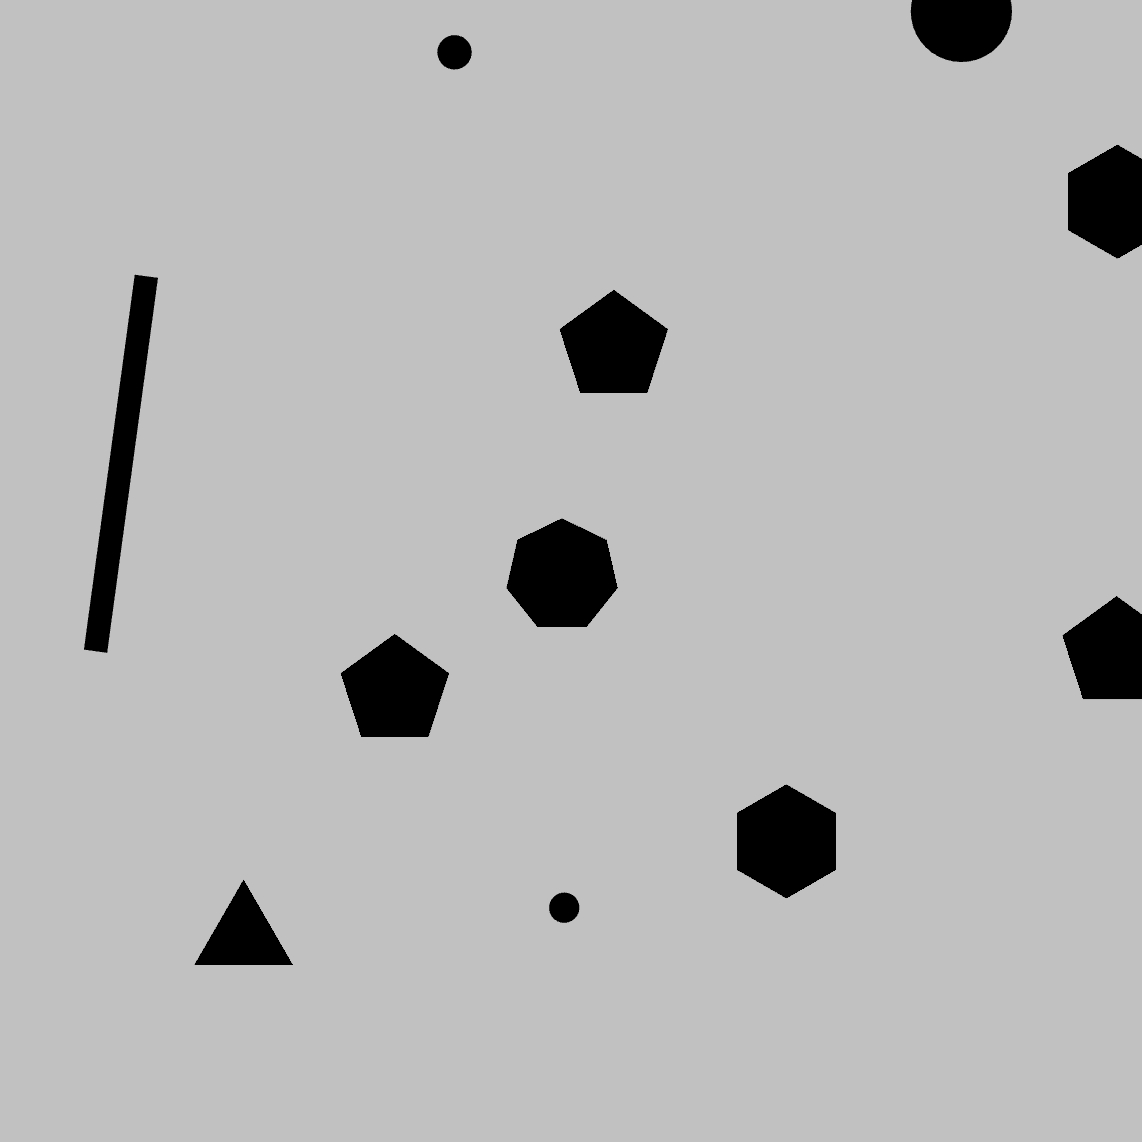
\includegraphics[width=\linewidth]{graphics/test_model_11_complex_1.png}
				\caption{Test worlds with 11 complex corrosion areas.}
				\label{fig:test_model_11_complex_1}
			\end{subfigure}
			\hfill
			\begin{subfigure}[t]{0.15\linewidth}
				\centering
				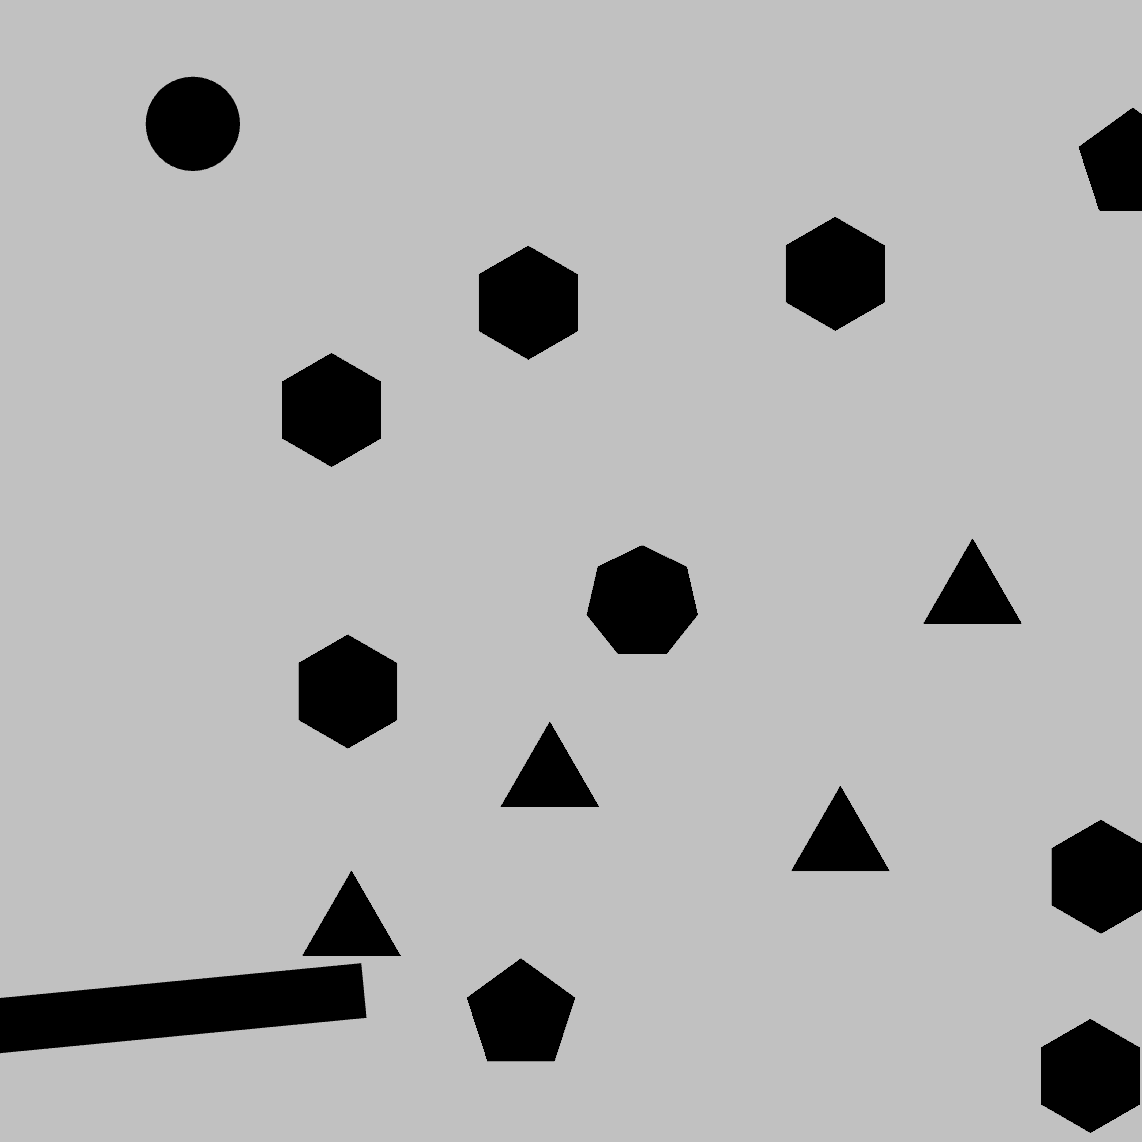
\includegraphics[width=\linewidth]{graphics/test_model_15_complex_1.png}
				\caption{Test worlds with 15 complex corrosion areas.}
				\label{fig:test_model_15_complex_1}
			\end{subfigure}
			\caption{Different test environments.}
			\label{fig:test_models}
		\end{figure}

	\chapter{Comparison of different navigation strategies}\label{annexe:comparaison}

		\begin{figure}[H]
			\begin{subfigure}[t]{0.9\linewidth}
				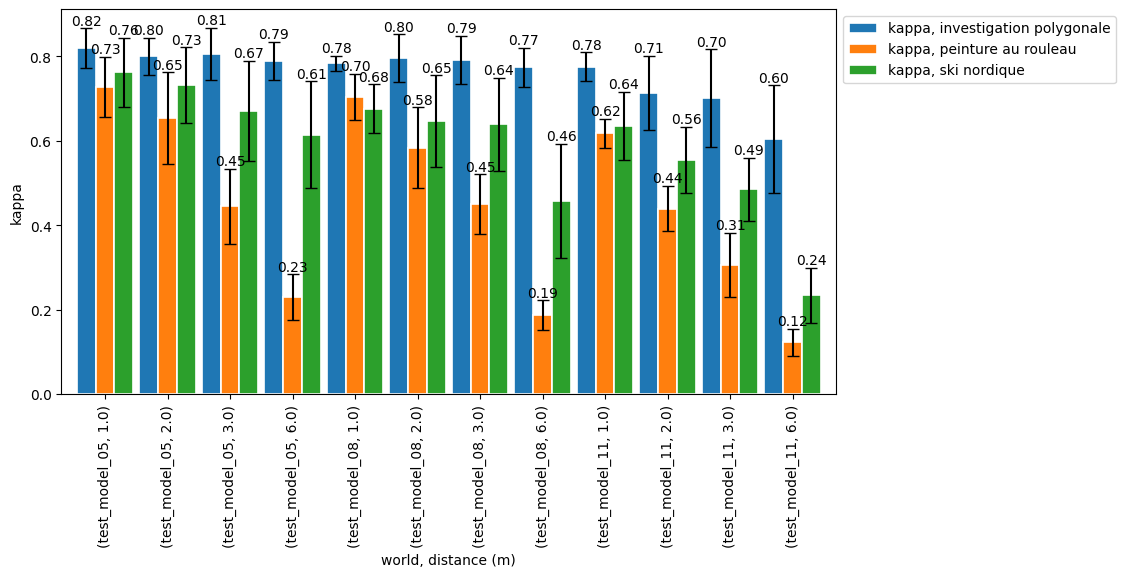
\includegraphics[width=\linewidth]{graphics/investigation_polygonale-peinture_au_rouleau_ski_nordique-kappa_for_each_d_vs_investigation_polygonale-kappa_for_each_d.png}
				\caption{$\kappa$ according to the density of the world.}
				\label{fig:investigation_polygonale-peinture_au_rouleau_ski_nordique-kappa_for_each_d_vs_investigation_polygonale-kappa_for_each_d}
			\end{subfigure}
			\hfill
			\begin{subfigure}[t]{0.9\linewidth}
				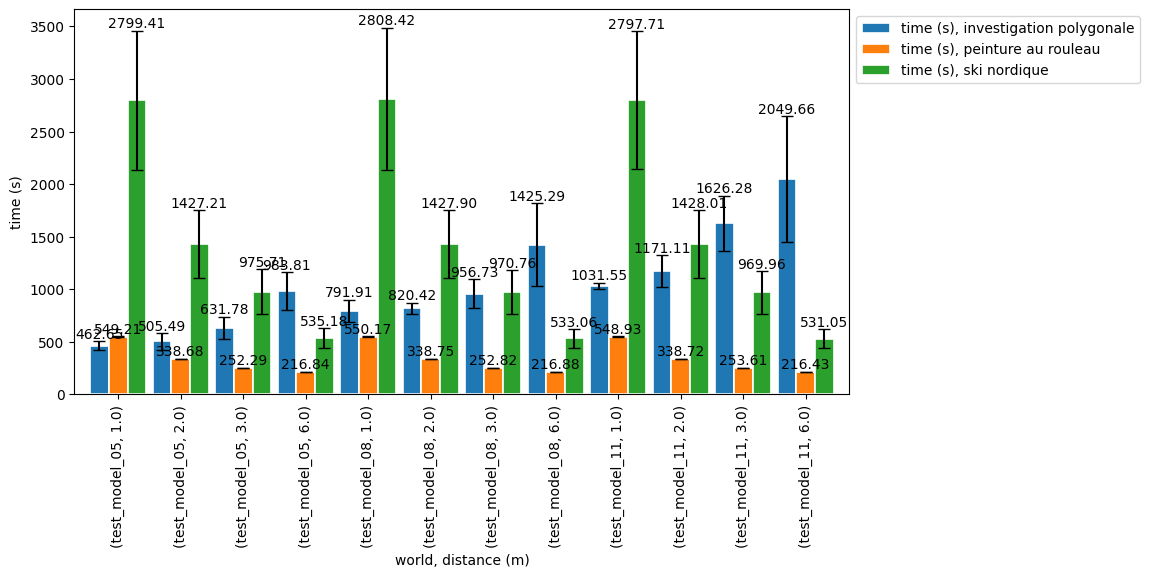
\includegraphics[width=\linewidth]{graphics/investigation_polygonale-peinture_au_rouleau_ski_nordique-time_for_each_d_vs_investigation_polygonale-time_for_each_d.png}
				\caption{Runtime based on world density.}
				\label{fig:investigation_polygonale-peinture_au_rouleau_ski_nordique-time_for_each_d_vs_investigation_polygonale-time_for_each_d}
			\end{subfigure}
			\caption{Evolution of Cohen's $\kappa$ and the execution time of the different algorithms according to the density of the world for different distances between the crawlers.}
			\label{fig:investigation_polygonale-peinture_au_rouleau_ski_nordique_for_each_d}
		\end{figure}

	\chapter{Investigation results}\label{annexe:resultat}

		\begin{figure}[H]
			\centering
			\begin{subfigure}[t]{\linewidth}
				\centering
				\begin{subfigure}[t]{0.12\linewidth}
					\includegraphics[width=\linewidth]{../tests/peinture_au_rouleau-test_model_05_1-1.0/both.png}
				\end{subfigure}
				\hfill
				\begin{subfigure}[t]{0.11\linewidth}
					\includegraphics[width=\linewidth]{../tests/peinture_au_rouleau-test_model_08_1-1.0/both.png}
				\end{subfigure}
				\hfill
				\begin{subfigure}[t]{0.11\linewidth}
					\includegraphics[width=\linewidth]{../tests/peinture_au_rouleau-test_model_11_1-1.0/both.png}
				\end{subfigure}
				\hfill
				\begin{subfigure}[t]{0.11\linewidth}
					\includegraphics[width=\linewidth]{../tests/peinture_au_rouleau-test_model_15_1-1.0/both.png}
				\end{subfigure}
				\hfill
				\begin{subfigure}[t]{0.11\linewidth}
					\includegraphics[width=\linewidth]{../tests/peinture_au_rouleau-test_model_20_1-1.0/both.png}
				\end{subfigure}
				\hfill
				\begin{subfigure}[t]{0.11\linewidth}
					\includegraphics[width=\linewidth]{../tests/peinture_au_rouleau-test_model_30_1-1.0/both.png}
				\end{subfigure}
				\hfill
				\begin{subfigure}[t]{0.11\linewidth}
					\includegraphics[width=\linewidth]{../tests/peinture_au_rouleau-test_model_11_complex_1-1.0/both.png}
				\end{subfigure}
				\hfill
				\begin{subfigure}[t]{0.11\linewidth}
					\includegraphics[width=\linewidth]{../tests/peinture_au_rouleau-test_model_15_complex_1-1.0/both.png}
				\end{subfigure}
				\caption{$d = 1$ m}
			\end{subfigure}
			\hfill
			\begin{subfigure}[t]{\linewidth}
				\centering
				\begin{subfigure}[t]{0.11\linewidth}
					\includegraphics[width=\linewidth]{../tests/peinture_au_rouleau-test_model_05_1-2.0/both.png}
				\end{subfigure}
				\hfill
				\begin{subfigure}[t]{0.11\linewidth}
					\includegraphics[width=\linewidth]{../tests/peinture_au_rouleau-test_model_08_1-2.0/both.png}
				\end{subfigure}
				\hfill
				\begin{subfigure}[t]{0.11\linewidth}
					\includegraphics[width=\linewidth]{../tests/peinture_au_rouleau-test_model_11_1-2.0/both.png}
				\end{subfigure}
				\hfill
				\begin{subfigure}[t]{0.11\linewidth}
					\includegraphics[width=\linewidth]{../tests/peinture_au_rouleau-test_model_15_1-2.0/both.png}
				\end{subfigure}
				\hfill
				\begin{subfigure}[t]{0.1\linewidth}
					\includegraphics[width=\linewidth]{../tests/peinture_au_rouleau-test_model_20_1-2.0/both.png}
				\end{subfigure}
				\hfill
				\begin{subfigure}[t]{0.11\linewidth}
					\includegraphics[width=\linewidth]{../tests/peinture_au_rouleau-test_model_30_1-2.0/both.png}
				\end{subfigure}
				\hfill
				\begin{subfigure}[t]{0.11\linewidth}
					\includegraphics[width=\linewidth]{../tests/peinture_au_rouleau-test_model_11_complex_1-2.0/both.png}
				\end{subfigure}
				\hfill
				\begin{subfigure}[t]{0.11\linewidth}
					\includegraphics[width=\linewidth]{../tests/peinture_au_rouleau-test_model_15_complex_1-2.0/both.png}
				\end{subfigure}
				\caption{$d = 2$ m}
			\end{subfigure}
			\hfill
			\begin{subfigure}[t]{\linewidth}
				\centering
				\begin{subfigure}[t]{0.11\linewidth}
					\includegraphics[width=\linewidth]{../tests/peinture_au_rouleau-test_model_05_1-3.0/both.png}
				\end{subfigure}
				\hfill
				\begin{subfigure}[t]{0.11\linewidth}
					\includegraphics[width=\linewidth]{../tests/peinture_au_rouleau-test_model_08_1-3.0/both.png}
				\end{subfigure}
				\hfill
				\begin{subfigure}[t]{0.11\linewidth}
					\includegraphics[width=\linewidth]{../tests/peinture_au_rouleau-test_model_11_1-3.0/both.png}
				\end{subfigure}
				\hfill
				\begin{subfigure}[t]{0.11\linewidth}
					\includegraphics[width=\linewidth]{../tests/peinture_au_rouleau-test_model_15_1-3.0/both.png}
				\end{subfigure}
				\hfill
				\begin{subfigure}[t]{0.11\linewidth}
					\includegraphics[width=\linewidth]{../tests/peinture_au_rouleau-test_model_20_1-3.0/both.png}
				\end{subfigure}
				\hfill
				\begin{subfigure}[t]{0.11\linewidth}
					\includegraphics[width=\linewidth]{../tests/peinture_au_rouleau-test_model_30_1-3.0/both.png}
				\end{subfigure}
				\hfill
				\begin{subfigure}[t]{0.11\linewidth}
					\includegraphics[width=\linewidth]{../tests/peinture_au_rouleau-test_model_11_complex_1-3.0/both.png}
				\end{subfigure}
				\hfill
				\begin{subfigure}[t]{0.11\linewidth}
					\includegraphics[width=\linewidth]{../tests/peinture_au_rouleau-test_model_15_complex_1-3.0/both.png}
				\end{subfigure}
				\caption{$d = 3$ m}
			\end{subfigure}
			\hfill
			\begin{subfigure}[t]{\linewidth}
				\centering
				\begin{subfigure}[t]{0.11\linewidth}
					\includegraphics[width=\linewidth]{../tests/peinture_au_rouleau-test_model_05_1-6.0/both.png}
				\end{subfigure}
				\hfill
				\begin{subfigure}[t]{0.11\linewidth}
					\includegraphics[width=\linewidth]{../tests/peinture_au_rouleau-test_model_08_1-6.0/both.png}
				\end{subfigure}
				\hfill
				\begin{subfigure}[t]{0.11\linewidth}
					\includegraphics[width=\linewidth]{../tests/peinture_au_rouleau-test_model_11_1-6.0/both.png}
				\end{subfigure}
				\hfill
				\begin{subfigure}[t]{0.11\linewidth}
					\includegraphics[width=\linewidth]{../tests/peinture_au_rouleau-test_model_15_1-6.0/both.png}
				\end{subfigure}
				\hfill
				\begin{subfigure}[t]{0.11\linewidth}
					\includegraphics[width=\linewidth]{../tests/peinture_au_rouleau-test_model_20_1-6.0/both.png}
				\end{subfigure}
				\hfill
				\begin{subfigure}[t]{0.11\linewidth}
					\includegraphics[width=\linewidth]{../tests/peinture_au_rouleau-test_model_30_1-6.0/both.png}
				\end{subfigure}
				\hfill
				\begin{subfigure}[t]{0.11\linewidth}
					\includegraphics[width=\linewidth]{../tests/peinture_au_rouleau-test_model_11_complex_1-6.0/both.png}
				\end{subfigure}
				\hfill
				\begin{subfigure}[t]{0.11\linewidth}
					\includegraphics[width=\linewidth]{../tests/peinture_au_rouleau-test_model_15_complex_1-6.0/both.png}
				\end{subfigure}
				\caption{$d = 6$ m}
			\end{subfigure}
			\caption{Overlay of the investigation maps with the mapping of the corrosion zones obtained for the different test worlds, for the \textit{Roller Painting} method.}
			\label{fig:peinture_au_rouleau_resultats}
		\end{figure}

		\begin{figure}[H]
			\centering
			\begin{subfigure}[t]{\linewidth}
				\centering
				\begin{subfigure}[t]{0.11\linewidth}
					\includegraphics[width=\linewidth]{../tests/ski_nordique-test_model_05_1-1.0-3.0/both.png}
				\end{subfigure}
				\hfill
				\begin{subfigure}[t]{0.11\linewidth}
					\includegraphics[width=\linewidth]{../tests/ski_nordique-test_model_08_1-1.0-3.0/both.png}
				\end{subfigure}
				\hfill
				\begin{subfigure}[t]{0.11\linewidth}
					\includegraphics[width=\linewidth]{../tests/ski_nordique-test_model_11_1-1.0-3.0/both.png}
				\end{subfigure}
				\hfill
				\begin{subfigure}[t]{0.11\linewidth}
					\includegraphics[width=\linewidth]{../tests/ski_nordique-test_model_15_1-1.0-3.0/both.png}
				\end{subfigure}
				\hfill
				\begin{subfigure}[t]{0.11\linewidth}
					\includegraphics[width=\linewidth]{../tests/ski_nordique-test_model_20_1-1.0-3.0/both.png}
				\end{subfigure}
				\hfill
				\begin{subfigure}[t]{0.11\linewidth}
					\includegraphics[width=\linewidth]{../tests/ski_nordique-test_model_30_1-1.0-3.0/both.png}
				\end{subfigure}
				\hfill
				\begin{subfigure}[t]{0.11\linewidth}
					\includegraphics[width=\linewidth]{../tests/ski_nordique-test_model_11_complex_1-1.0-3.0/both.png}
				\end{subfigure}
				\hfill
				\begin{subfigure}[t]{0.11\linewidth}
					\includegraphics[width=\linewidth]{../tests/ski_nordique-test_model_15_complex_1-1.0-3.0/both.png}
				\end{subfigure}
				\caption{$d = 1$ m, $s = 3$ m}
			\end{subfigure}
			\hfill
			\begin{subfigure}[t]{\linewidth}
				\centering
				\begin{subfigure}[t]{0.11\linewidth}
					\includegraphics[width=\linewidth]{../tests/ski_nordique-test_model_05_1-2.0-3.0/both.png}
				\end{subfigure}
				\hfill
				\begin{subfigure}[t]{0.11\linewidth}
					\includegraphics[width=\linewidth]{../tests/ski_nordique-test_model_08_1-2.0-3.0/both.png}
				\end{subfigure}
				\hfill
				\begin{subfigure}[t]{0.11\linewidth}
					\includegraphics[width=\linewidth]{../tests/ski_nordique-test_model_11_1-2.0-3.0/both.png}
				\end{subfigure}
				\hfill
				\begin{subfigure}[t]{0.11\linewidth}
					\includegraphics[width=\linewidth]{../tests/ski_nordique-test_model_15_1-2.0-3.0/both.png}
				\end{subfigure}
				\hfill
				\begin{subfigure}[t]{0.11\linewidth}
					\includegraphics[width=\linewidth]{../tests/ski_nordique-test_model_20_1-2.0-3.0/both.png}
				\end{subfigure}
				\hfill
				\begin{subfigure}[t]{0.11\linewidth}
					\includegraphics[width=\linewidth]{../tests/ski_nordique-test_model_30_1-2.0-3.0/both.png}
				\end{subfigure}
				\hfill
				\begin{subfigure}[t]{0.11\linewidth}
					\includegraphics[width=\linewidth]{../tests/ski_nordique-test_model_11_complex_1-2.0-3.0/both.png}
				\end{subfigure}
				\hfill
				\begin{subfigure}[t]{0.11\linewidth}
					\includegraphics[width=\linewidth]{../tests/ski_nordique-test_model_15_complex_1-2.0-3.0/both.png}
				\end{subfigure}
				\caption{$d = 2$ m, $s = 3$ m}
			\end{subfigure}
			\hfill
			\begin{subfigure}[t]{\linewidth}
				\centering
				\begin{subfigure}[t]{0.11\linewidth}
					\includegraphics[width=\linewidth]{../tests/ski_nordique-test_model_05_1-3.0-3.0/both.png}
				\end{subfigure}
				\hfill
				\begin{subfigure}[t]{0.11\linewidth}
					\includegraphics[width=\linewidth]{../tests/ski_nordique-test_model_08_1-3.0-3.0/both.png}
				\end{subfigure}
				\hfill
				\begin{subfigure}[t]{0.11\linewidth}
					\includegraphics[width=\linewidth]{../tests/ski_nordique-test_model_11_1-3.0-3.0/both.png}
				\end{subfigure}
				\hfill
				\begin{subfigure}[t]{0.11\linewidth}
					\includegraphics[width=\linewidth]{../tests/ski_nordique-test_model_15_1-3.0-3.0/both.png}
				\end{subfigure}
				\hfill
				\begin{subfigure}[t]{0.11\linewidth}
					\includegraphics[width=\linewidth]{../tests/ski_nordique-test_model_20_1-3.0-3.0/both.png}
				\end{subfigure}
				\hfill
				\begin{subfigure}[t]{0.11\linewidth}
					\includegraphics[width=\linewidth]{../tests/ski_nordique-test_model_30_1-3.0-3.0/both.png}
				\end{subfigure}
				\hfill
				\begin{subfigure}[t]{0.11\linewidth}
					\includegraphics[width=\linewidth]{../tests/ski_nordique-test_model_11_complex_1-3.0-3.0/both.png}
				\end{subfigure}
				\hfill
				\begin{subfigure}[t]{0.11\linewidth}
					\includegraphics[width=\linewidth]{../tests/ski_nordique-test_model_15_complex_1-3.0-3.0/both.png}
				\end{subfigure}
				\caption{$d = 3$ m, $s = 3$ m}
			\end{subfigure}
			\hfill
			\begin{subfigure}[t]{\linewidth}
				\centering
				\begin{subfigure}[t]{0.11\linewidth}
					\includegraphics[width=\linewidth]{../tests/ski_nordique-test_model_05_1-6.0-3.0/both.png}
				\end{subfigure}
				\hfill
				\begin{subfigure}[t]{0.11\linewidth}
					\includegraphics[width=\linewidth]{../tests/ski_nordique-test_model_08_1-6.0-3.0/both.png}
				\end{subfigure}
				\hfill
				\begin{subfigure}[t]{0.11\linewidth}
					\includegraphics[width=\linewidth]{../tests/ski_nordique-test_model_11_1-6.0-3.0/both.png}
				\end{subfigure}
				\hfill
				\begin{subfigure}[t]{0.11\linewidth}
					\includegraphics[width=\linewidth]{../tests/ski_nordique-test_model_15_1-6.0-3.0/both.png}
				\end{subfigure}
				\hfill
				\begin{subfigure}[t]{0.11\linewidth}
					\includegraphics[width=\linewidth]{../tests/ski_nordique-test_model_20_1-6.0-3.0/both.png}
				\end{subfigure}
				\hfill
				\begin{subfigure}[t]{0.11\linewidth}
					\includegraphics[width=\linewidth]{../tests/ski_nordique-test_model_30_1-6.0-3.0/both.png}
				\end{subfigure}
				\hfill
				\begin{subfigure}[t]{0.11\linewidth}
					\includegraphics[width=\linewidth]{../tests/ski_nordique-test_model_11_complex_1-6.0-3.0/both.png}
				\end{subfigure}
				\hfill
				\begin{subfigure}[t]{0.11\linewidth}
					\includegraphics[width=\linewidth]{../tests/ski_nordique-test_model_15_complex_1-6.0-3.0/both.png}
				\end{subfigure}
				\caption{$d = 6$ m, $s = 3$ m}
			\end{subfigure}
			\caption{Overlay of the investigation maps with the mapping of the corrosion zones obtained for the different test worlds, for the \textit{Nordic Skiing} method - 1.}
			\label{fig:ski_nordique_resultats}
		\end{figure}

		\begin{figure}[H]
			\centering
			\begin{subfigure}[t]{\linewidth}
				\centering
				\begin{subfigure}[t]{0.11\linewidth}
					\includegraphics[width=\linewidth]{../tests/ski_nordique-test_model_05_1-3.0-1.0/both.png}
				\end{subfigure}
				\hfill
				\begin{subfigure}[t]{0.11\linewidth}
					\includegraphics[width=\linewidth]{../tests/ski_nordique-test_model_08_1-3.0-1.0/both.png}
				\end{subfigure}
				\hfill
				\begin{subfigure}[t]{0.11\linewidth}
					\includegraphics[width=\linewidth]{../tests/ski_nordique-test_model_11_1-3.0-1.0/both.png}
				\end{subfigure}
				\hfill
				\begin{subfigure}[t]{0.11\linewidth}
					\includegraphics[width=\linewidth]{../tests/ski_nordique-test_model_15_1-3.0-1.0/both.png}
				\end{subfigure}
				\hfill
				\begin{subfigure}[t]{0.11\linewidth}
					\includegraphics[width=\linewidth]{../tests/ski_nordique-test_model_20_1-3.0-1.0/both.png}
				\end{subfigure}
				\hfill
				\begin{subfigure}[t]{0.11\linewidth}
					\includegraphics[width=\linewidth]{../tests/ski_nordique-test_model_30_1-3.0-1.0/both.png}
				\end{subfigure}
				\hfill
				\begin{subfigure}[t]{0.11\linewidth}
					\includegraphics[width=\linewidth]{../tests/ski_nordique-test_model_11_complex_1-3.0-1.0/both.png}
				\end{subfigure}
				\hfill
				\begin{subfigure}[t]{0.11\linewidth}
					\includegraphics[width=\linewidth]{../tests/ski_nordique-test_model_15_complex_1-3.0-1.0/both.png}
				\end{subfigure}
				\caption{$d = 3$ m, $s = 1$ m}
			\end{subfigure}
			\hfill
			\begin{subfigure}[t]{\linewidth}
				\centering
				\begin{subfigure}[t]{0.11\linewidth}
					\includegraphics[width=\linewidth]{../tests/ski_nordique-test_model_05_1-3.0-2.0/both.png}
				\end{subfigure}
				\hfill
				\begin{subfigure}[t]{0.11\linewidth}
					\includegraphics[width=\linewidth]{../tests/ski_nordique-test_model_08_1-3.0-2.0/both.png}
				\end{subfigure}
				\hfill
				\begin{subfigure}[t]{0.11\linewidth}
					\includegraphics[width=\linewidth]{../tests/ski_nordique-test_model_11_1-3.0-2.0/both.png}
				\end{subfigure}
				\hfill
				\begin{subfigure}[t]{0.11\linewidth}
					\includegraphics[width=\linewidth]{../tests/ski_nordique-test_model_15_1-3.0-2.0/both.png}
				\end{subfigure}
				\hfill
				\begin{subfigure}[t]{0.11\linewidth}
					\includegraphics[width=\linewidth]{../tests/ski_nordique-test_model_20_1-3.0-2.0/both.png}
				\end{subfigure}
				\hfill
				\begin{subfigure}[t]{0.11\linewidth}
					\includegraphics[width=\linewidth]{../tests/ski_nordique-test_model_30_1-3.0-2.0/both.png}
				\end{subfigure}
				\hfill
				\begin{subfigure}[t]{0.11\linewidth}
					\includegraphics[width=\linewidth]{../tests/ski_nordique-test_model_11_complex_1-3.0-2.0/both.png}
				\end{subfigure}
				\hfill
				\begin{subfigure}[t]{0.11\linewidth}
					\includegraphics[width=\linewidth]{../tests/ski_nordique-test_model_15_complex_1-3.0-2.0/both.png}
				\end{subfigure}
				\caption{$d = 3$ m, $s = 2$ m}
			\end{subfigure}
			\hfill
			\begin{subfigure}[t]{\linewidth}
				\centering
				\begin{subfigure}[t]{0.11\linewidth}
					\includegraphics[width=\linewidth]{../tests/ski_nordique-test_model_05_1-3.0-3.0/both.png}
				\end{subfigure}
				\hfill
				\begin{subfigure}[t]{0.11\linewidth}
					\includegraphics[width=\linewidth]{../tests/ski_nordique-test_model_08_1-3.0-3.0/both.png}
				\end{subfigure}
				\hfill
				\begin{subfigure}[t]{0.11\linewidth}
					\includegraphics[width=\linewidth]{../tests/ski_nordique-test_model_11_1-3.0-3.0/both.png}
				\end{subfigure}
				\hfill
				\begin{subfigure}[t]{0.11\linewidth}
					\includegraphics[width=\linewidth]{../tests/ski_nordique-test_model_15_1-3.0-3.0/both.png}
				\end{subfigure}
				\hfill
				\begin{subfigure}[t]{0.11\linewidth}
					\includegraphics[width=\linewidth]{../tests/ski_nordique-test_model_20_1-3.0-3.0/both.png}
				\end{subfigure}
				\hfill
				\begin{subfigure}[t]{0.11\linewidth}
					\includegraphics[width=\linewidth]{../tests/ski_nordique-test_model_30_1-3.0-3.0/both.png}
				\end{subfigure}
				\hfill
				\begin{subfigure}[t]{0.11\linewidth}
					\includegraphics[width=\linewidth]{../tests/ski_nordique-test_model_11_complex_1-3.0-3.0/both.png}
				\end{subfigure}
				\hfill
				\begin{subfigure}[t]{0.11\linewidth}
					\includegraphics[width=\linewidth]{../tests/ski_nordique-test_model_15_complex_1-3.0-3.0/both.png}
				\end{subfigure}
				\caption{$d = 3$ m, $s = 3$ m}
			\end{subfigure}
			\hfill
			\begin{subfigure}[t]{\linewidth}
				\centering
				\begin{subfigure}[t]{0.11\linewidth}
					\includegraphics[width=\linewidth]{../tests/ski_nordique-test_model_05_1-3.0-6.0/both.png}
				\end{subfigure}
				\hfill
				\begin{subfigure}[t]{0.11\linewidth}
					\includegraphics[width=\linewidth]{../tests/ski_nordique-test_model_08_1-3.0-6.0/both.png}
				\end{subfigure}
				\hfill
				\begin{subfigure}[t]{0.11\linewidth}
					\includegraphics[width=\linewidth]{../tests/ski_nordique-test_model_11_1-3.0-6.0/both.png}
				\end{subfigure}
				\hfill
				\begin{subfigure}[t]{0.11\linewidth}
					\includegraphics[width=\linewidth]{../tests/ski_nordique-test_model_15_1-3.0-6.0/both.png}
				\end{subfigure}
				\hfill
				\begin{subfigure}[t]{0.11\linewidth}
					\includegraphics[width=\linewidth]{../tests/ski_nordique-test_model_20_1-3.0-6.0/both.png}
				\end{subfigure}
				\hfill
				\begin{subfigure}[t]{0.11\linewidth}
					\includegraphics[width=\linewidth]{../tests/ski_nordique-test_model_30_1-3.0-6.0/both.png}
				\end{subfigure}
				\hfill
				\begin{subfigure}[t]{0.11\linewidth}
					\includegraphics[width=\linewidth]{../tests/ski_nordique-test_model_11_complex_1-3.0-6.0/both.png}
				\end{subfigure}
				\hfill
				\begin{subfigure}[t]{0.11\linewidth}
					\includegraphics[width=\linewidth]{../tests/ski_nordique-test_model_15_complex_1-3.0-6.0/both.png}
				\end{subfigure}
				\caption{$d = 6$ m, $s = 3$ m}
			\end{subfigure}
			\caption{Overlay of the investigation maps with the mapping of the corrosion zones obtained for the different test worlds, for the \textit{Nordic Skiing} method - 2.}
			\label{fig:ski_nordique_resultats_2}
		\end{figure}

		\begin{figure}[H]
			\centering
			\begin{subfigure}[t]{\linewidth}
				\centering
				\begin{subfigure}[t]{0.2\linewidth}
					\includegraphics[width=\linewidth]{../tests/investigation_polygonale-test_model_05_1-4-2-1.0/both.png}
				\end{subfigure}
				\hfill
				\begin{subfigure}[t]{0.2\linewidth}
					\includegraphics[width=\linewidth]{../tests/investigation_polygonale-test_model_08_1-4-2-1.0/both.png}
				\end{subfigure}
				\hfill
				\begin{subfigure}[t]{0.2\linewidth}
					\includegraphics[width=\linewidth]{../tests/investigation_polygonale-test_model_11_1-4-2-1.0/both.png}
				\end{subfigure}
				\caption{$k = 1$, $n = 2$, $p = 4$, $d = 1$ m}
			\end{subfigure}
			\hfill
			\begin{subfigure}[t]{\linewidth}
				\centering
				\begin{subfigure}[t]{0.2\linewidth}
					\includegraphics[width=\linewidth]{../tests/investigation_polygonale-test_model_05_1-4-2-2.0/both.png}
				\end{subfigure}
				\hfill
				\begin{subfigure}[t]{0.2\linewidth}
					\includegraphics[width=\linewidth]{../tests/investigation_polygonale-test_model_08_1-4-2-2.0/both.png}
				\end{subfigure}
				\hfill
				\begin{subfigure}[t]{0.2\linewidth}
					\includegraphics[width=\linewidth]{../tests/investigation_polygonale-test_model_11_1-4-2-2.0/both.png}
				\end{subfigure}
				\caption{$k = 1$, $n = 2$, $p = 4$, $d = 2$ m}
			\end{subfigure}
			\hfill
			\begin{subfigure}[t]{\linewidth}
				\centering
				\begin{subfigure}[t]{0.2\linewidth}
					\includegraphics[width=\linewidth]{../tests/investigation_polygonale-test_model_05_1-4-2-3.0/both.png}
				\end{subfigure}
				\hfill
				\begin{subfigure}[t]{0.2\linewidth}
					\includegraphics[width=\linewidth]{../tests/investigation_polygonale-test_model_08_1-4-2-3.0/both.png}
				\end{subfigure}
				\hfill
				\begin{subfigure}[t]{0.2\linewidth}
					\includegraphics[width=\linewidth]{../tests/investigation_polygonale-test_model_11_1-4-2-3.0/both.png}
				\end{subfigure}
				\caption{$k = 1$, $n = 2$, $p = 4$, $d = 3$ m}
			\end{subfigure}
			\hfill
			\begin{subfigure}[t]{\linewidth}
				\centering
				\begin{subfigure}[t]{0.2\linewidth}
					\includegraphics[width=\linewidth]{../tests/investigation_polygonale-test_model_05_1-4-2-6.0/both.png}
				\end{subfigure}
				\hfill
				\begin{subfigure}[t]{0.2\linewidth}
					\includegraphics[width=\linewidth]{../tests/investigation_polygonale-test_model_08_1-4-2-6.0/both.png}
				\end{subfigure}
				\hfill
				\begin{subfigure}[t]{0.2\linewidth}
					\includegraphics[width=\linewidth]{../tests/investigation_polygonale-test_model_11_1-4-2-6.0/both.png}
				\end{subfigure}
				\caption{$k = 1$, $n = 2$, $p = 4$, $d = 6$ m}
			\end{subfigure}
			\caption{Overlay of the investigation maps with the map of the corrosion zones obtained for the different test worlds, for the \textit{Polygonal Investigation} method - 1.}
			\label{fig:investigation_polygonale_resultats}
		\end{figure}

		\begin{figure}[H]
			\centering
			\begin{subfigure}[t]{\linewidth}
				\centering
				\begin{subfigure}[t]{0.2\linewidth}
					\includegraphics[width=\linewidth]{../tests/investigation_polygonale-test_model_05_1-6-2-1.0/both.png}
				\end{subfigure}
				\caption{$k = 1$, $n = 2$, $p = 6$, $d = 1$ m}
			\end{subfigure}
			\hfill
			\begin{subfigure}[t]{\linewidth}
				\centering
				\begin{subfigure}[t]{0.2\linewidth}
					\includegraphics[width=\linewidth]{../tests/investigation_polygonale-test_model_05_1-6-2-2.0/both.png}
				\end{subfigure}
				\caption{$k = 1$, $n = 2$, $p = 6$, $d = 2$ m}
			\end{subfigure}
			\hfill
			\begin{subfigure}[t]{\linewidth}
				\centering
				\begin{subfigure}[t]{0.2\linewidth}
					\includegraphics[width=\linewidth]{../tests/investigation_polygonale-test_model_05_1-6-2-3.0/both.png}
				\end{subfigure}
				\caption{$k = 1$, $n = 2$, $p = 6$, $d = 3$ m}
			\end{subfigure}
			\hfill
			\begin{subfigure}[t]{\linewidth}
				\centering
				\begin{subfigure}[t]{0.2\linewidth}
					\includegraphics[width=\linewidth]{../tests/investigation_polygonale-test_model_05_1-6-2-6.0/both.png}
				\end{subfigure}
				\caption{$k = 1$, $n = 2$, $p = 6$, $d = 6$ m}
			\end{subfigure}
			\caption{Overlay of the investigation maps with the mapping of the corrosion zones obtained for the different test worlds, for the \textit{Polygonal Investigation} method - 2.}
			\label{fig:investigation_polygonale_resultats_2}
		\end{figure}

\end{theappendices}

